% !TeX spellcheck = cs_CZ
{\tikzset{external/prefix={tikz/FYZII/}}
 \tikzset{external/figure name/.add={ch14_}{}}
%---------------------------------------------------------------------------------------------------
% file fey2ch14.tex
%---------------------------------------------------------------------------------------------------
%====================Kapitola: Magnetické pole v různých případech =================================
\chapter{Magnetické pole v různých případech}\label{fyz:IIchapXIV}
\minitoc

  \section{Vektorový potenciál}\label{fyz:IIchapXIVsecI}
  \section{Vektorový potenciál daných proudů}\label{fyz:IIchapXIVsecII}
  \section{Přímý vodič}\label{fyz:IIchapXIVsecIII}
  \section{Dlouhý solenoid}\label{fyz:IIchapXIVsecIV}
  \section{Pole malé smyčky. Magnetický dipól}\label{fyz:IIchapXIVsecV}
  \section{Vektorový potenciál obvodu}\label{fyz:IIchapXIVsecVI}
  \section{Biot-Savartův zákon}\label{fyz:IIchapXIVsecVII}

    \begin{figure}[ht!] %\ref{fyz_fig673}
      \centering
      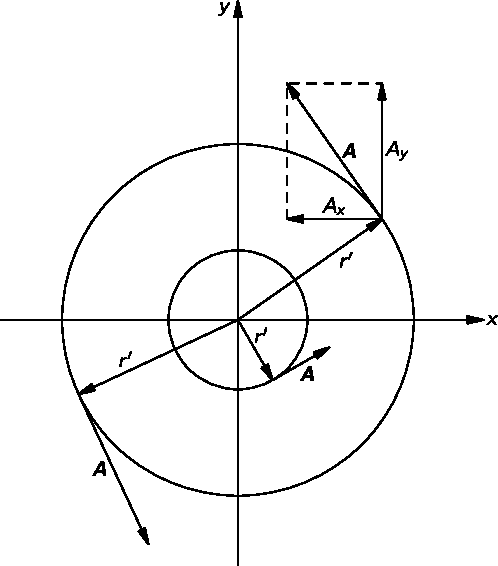
\includegraphics[width=0.7\linewidth]{fyz_fig673.pdf}
      \caption{
               (\cite[s.~707]{Feynman02})}
      \label{fyz_fig673}
    \end{figure}

    \begin{figure}[ht!] %\ref{fyz_fig674}
      \centering
      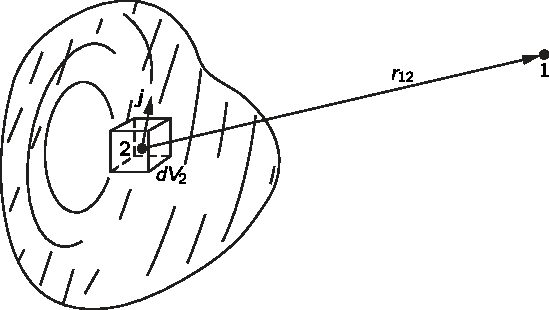
\includegraphics[width=0.7\linewidth]{fyz_fig674.pdf}
      \caption{
               (\cite[s.~707]{Feynman02})}
      \label{fyz_fig674}
    \end{figure}

    \begin{figure}[ht!] %\ref{fyz_fig675}
      \centering
      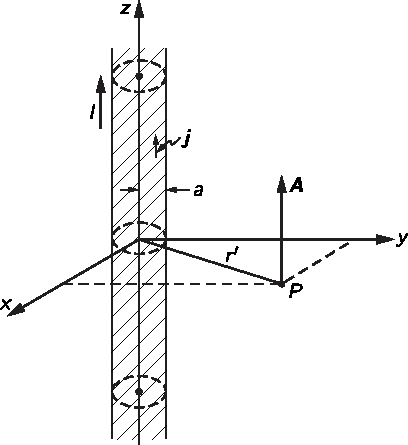
\includegraphics[width=0.7\linewidth]{fyz_fig675.pdf}
      \caption{
               (\cite[s.~707]{Feynman02})}
      \label{fyz_fig675}
    \end{figure}

    \begin{figure}[ht!] %\ref{fyz_fig676}
      \centering
      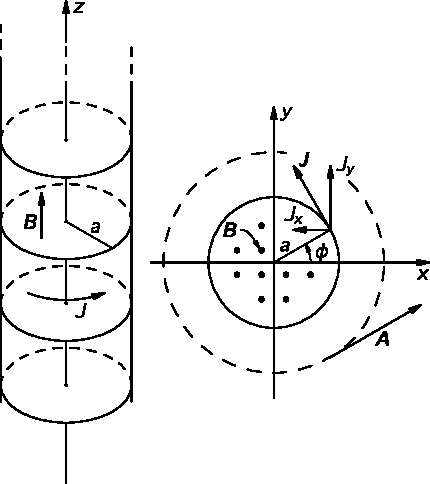
\includegraphics[width=0.7\linewidth]{fyz_fig676.pdf}
      \caption{
               (\cite[s.~707]{Feynman02})}
      \label{fyz_fig676}
    \end{figure}
    
    \begin{figure}[ht!] %\ref{fyz_fig677}
      \centering
      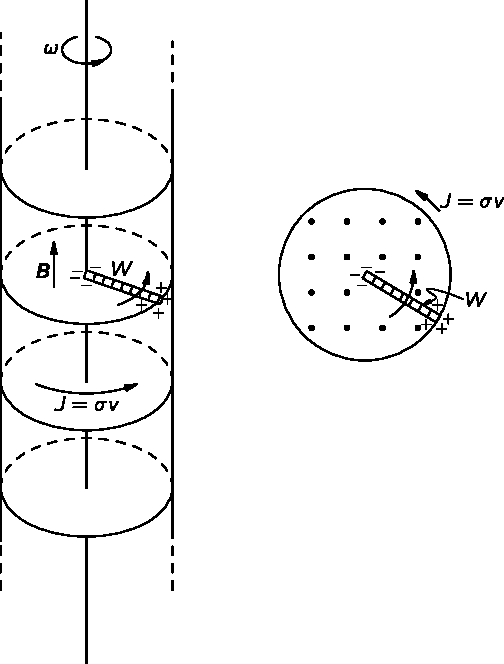
\includegraphics[width=0.7\linewidth]{fyz_fig677.pdf}
      \caption{
               (\cite[s.~707]{Feynman02})}
      \label{fyz_fig677}
    \end{figure}

    \begin{figure}[ht!] %\ref{fyz_fig678}
      \centering
      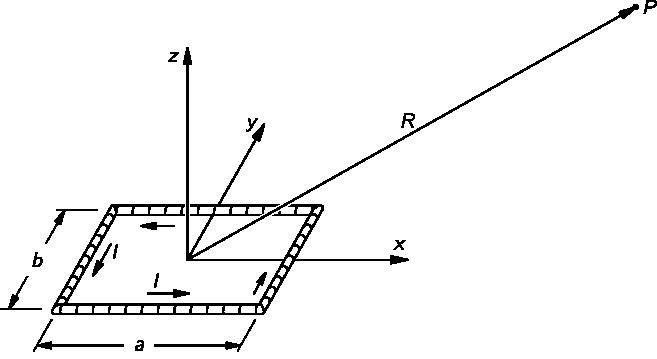
\includegraphics[width=0.7\linewidth]{fyz_fig678.pdf}
      \caption{
               (\cite[s.~707]{Feynman02})}
      \label{fyz_fig678}
    \end{figure}

    \begin{figure}[ht!] %\ref{fyz_fig679}
      \centering
      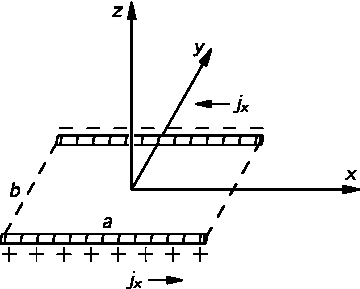
\includegraphics[width=0.7\linewidth]{fyz_fig679.pdf}
      \caption{
               (\cite[s.~707]{Feynman02})}
      \label{fyz_fig679}
    \end{figure}

    \begin{figure}[ht!] %\ref{fyz_fig680}
      \centering
      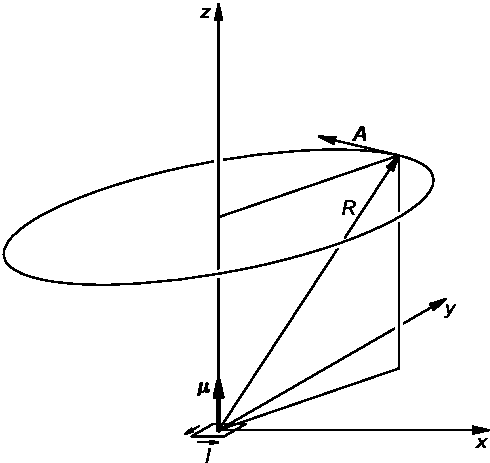
\includegraphics[width=0.7\linewidth]{fyz_fig680.pdf}
      \caption{
               (\cite[s.~707]{Feynman02})}
      \label{fyz_fig680}
    \end{figure}

    \begin{figure}[ht!] %\ref{fyz_fig681}
      \centering
      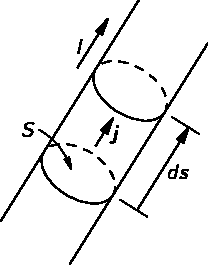
\includegraphics[width=0.5\linewidth]{fyz_fig681.pdf}
      \caption{
               (\cite[s.~707]{Feynman02})}
      \label{fyz_fig681}
    \end{figure}

    \begin{figure}[ht!] %\ref{fyz_fig682}
      \centering
      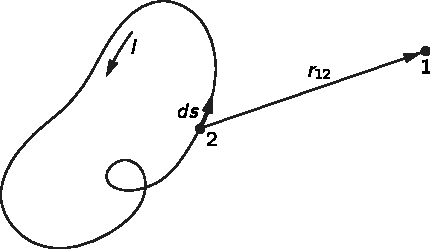
\includegraphics[width=0.7\linewidth]{fyz_fig682.pdf}
      \caption{
               (\cite[s.~707]{Feynman02})}
      \label{fyz_fig682}
    \end{figure}



} %tikzset
%~~~~~~~~~~~~~~~~~~~~~~~~~~~~~~~~~~~~~~~~~~~~~~~~~~~~~~~~~~~~~~~~~~~~~~~~~~~~~~~~~~~~~~~~~~~~~~~~~~
\printbibliography[title={Seznam literatury}, heading=subbibliography]
\addcontentsline{toc}{section}{Seznam literatury}